
%%%%%%%%%%%%%%%%%%%%%%% file sese_vorlage.tex %%%%%%%%%%%%%%%%%%%%%%%%%
%
% LaTex Beispiel für das Seminar Software Engineering.
% Enthält super interessante und wichtige Bearbeitungshinweise.
%
% Vorlage basiert auf der Springer LNCS Vorlage und ist nur
% für Seminararbeiten an der Universität Würzburg zu verwenden.
%
%%%%%%%%%%%%%%%%%%%%%%%%%%%%%%%%%%%%%%%%%%%%%%%%%%%%%%%%%%%%%%%%%%%


\documentclass[runningheads,a4paper]{uwsese}


%% -------------------------------
%% | Information for Declaration |
%% -------------------------------
\newcommand{\authorName}{Ștefan-Octavian Radu}
\newcommand{\place}{Würzburg}
\newcommand{\submissionTime}{29 January 2024}


\usepackage[utf8]{inputenc}
\usepackage{amssymb}
\usepackage{amsmath}
\setcounter{tocdepth}{3}
\usepackage{graphicx}
\graphicspath{ {./graphics/} }
\usepackage{array}
\usepackage{ragged2e}
\usepackage{arydshln}
\usepackage{xcolor}
\usepackage{parskip}
\newcolumntype{P}[1]{>{\RaggedRight\hspace{0pt}}p{#1}}
%\newcolumntype{P}[1]{>{\raggedright\arraybackslash}p{#1}}


\usepackage{url}
\urldef{\mailsa}\path|dozent.ls2.informatik@uni-wuerzburg.de| 
\newcommand{\keywords}[1]{\par\addvspace\baselineskip
\noindent\keywordname\enspace\ignorespaces#1}

\begin{document}

\mainmatter 

% first the title is needed
\title{Trusted Execution Environments: An Overview}
\subtitle{Seminar Software Engineering}

% a short form should be given in case it is too long for the running head
%\titlerunning{Bearbeitungshinweise Seminar Software Engineering}
%\titlerunning{} %TODO

\date{Winter Semester 2023}


\author{Ștefan-Octavian Radu}
%
%\authorrunning{LS2 Dozent}
%\authorrunning{Trusted Execution Environments: An Overview} %TODO
% (feature abused for this document to repeat the title also on left hand pages)

% the affiliations are given next
\institute{University of W\"urzburg,
Germany\\
\mailsa\\
}

\maketitle

\begin{abstract}

    With computing systems processing more and more information, arose the need
    for more rigorous security guarantees for the processed data. Trusted
    execution environments (TEE) are one of the solutions which address the
    problem of secure computation. They enable secure code execution and data
    storage in a secure isolated execution environment. In this paper we will
    cover the architecture of these systems, how they are currently used, both
    in the industry and in academia, and what tools are available for
    application development. In the end we will cover some known attacks that
    have been proven to compromise the security guarantees of TEE.

\end{abstract}

\section{Introduction}

The computing systems of the present are more and more complex. Their
applications range from personal computers and mobile phones targeting end
users, to large-scale servers dedicated to processing large amounts of data in
the cloud. As computers became more capable in the recent years, more and more
sensitive information started to pass through these systems. In order to
protect this data, some security mechanisms had to be implemented. This is a
difficult task because of the sheer complexity of computing systems themselves,
as well as the large number of software components that run simultaneously on a
system, each of which does not come with any security guarantee and issues
within it can affect the security of the other components. 

On of the most widely used solutions for the isolation of sensitive information
is the use of Trusted Execution Environments (TEE). These are usually based on some
hardware extensions that enable the creation of execution contexts, completely
isolated from the rest of the system. By making use of such isolated
environments to make sensitive computations, the trust is moved away from other
software components that coexist on the computing platform or the operating
system itself, exclusively to the primitives that make such isolation possible.

This paper we will give an overview of Trusted Execution Environments, starting
with a definition and covering some key terms. We will then discuss in detail
the architecture and the security principles that make them possible, including
chains of trust from initialisation until the instantiation of such an
environment, memory protection of various components during runtime, the secure
storage of information across instances and how secure interaction with
external IO devices can be performed. Further, the main applications of TEEs we 
will cover the main applications of a TEE, the array of tooling available for
the development of applications for TEEs as well as common difficulties in the 
current development process. Lastly we will cover security vulnerabilities which
have been found in TEEs since their adoption, thus highlighting some shortcomings
of the technology.

\section{Background}

This short section will give an overview of a few important concepts present
throughout this material, as well as a definition of Trusted Execution
Environments.

\subsection{Definition}

A \emph{Trusted execution environment} is a feature of modern microprocessors
which provides a hardware-isolated ``secure area that runs in parallel with,
but separate, from the normal execution environment'' \cite{tee_ieee_standard}.
This environment aims to guarantee that the executed code, the runtime states
and the stored data are integrity and privacy protected. It's end goal is to
improve the overall security of the whole system (\cite{tee_app_rev},
\cite{tee_in_securities}, \cite{tee_is_and_not}).

It is important to note that definitions of TEEs vary in literature. The above is
not an official definition, but rather a combination of core ideas extracted from
multiple sources with the goal of covering all the core ideas of the subject.

\subsection{Key Terms}

\subsubsection{Enclave.}

Even thought \emph{enclaves} are often confused or used interchangeably with
TEEs, those terms are subtly different. As defined in the \emph{IEEE standard}
\cite{tee_ieee_standard}, an enclave is a protected memory area, the contents
of which cannot be tampered with, or read from outside the enclave. Most often,
enclaves are instances of TEEs, while TEEs are the entire set of technologies
that enable the creation of enclaves.

\subsubsection{Mutability.}

In this context, we refer to a component of the TCB as being \emph{mutable}
when it can be updated post-manufacturing. Mutable components are usually
implemented in software, but there are exceptions, such as CPU microcode
\cite{microcode_update}. \emph{Immutable} components cannot be changed after
manufacturing, are most commonly implemented in hardware and are prevalent as
\emph{Root of Trust} (see \ref{rot}) (eg. PUF \cite{tee_base_article}).
Software can be also immutable (eg. Boot ROM as part of Secure Boot).

\subsubsection{Trusted Computer Base.}

``The hardware and software components that are used to achieve the security
protections of a TEE is called the Trusted Computing Base (TCB)''
\cite{tee_hw_sup}. Most often, it is desirable to minimize the TCB, thus
reducing the possible number of bugs and vulnerabilities and making it more
suitable to be formally verified. However, many solutions choose to have
mutable components as part of the TCB, which enables updating it down the line,
instead of relying on formal methods to guarantee safety. This will be further
highlighted when discussing the security principles of the most common TEE
implementations.

\subsubsection{Trusted Applications.}

The code that is executed inside a TEEs is commonly referred to as a
\emph{Trusted Application}, although it typically is just a small portion of a
larger application that handles sensitive data \cite{tee_app_rev}.

\subsubsection{Trusted Platform Module.}

The Trusted Platform Module (TPM) can either refer to an international standard
for a microcontroller designed to enable trust in computing platforms by
securing hardware through integrated cryptographic keys, or to specific chips 
which follow this standard \cite{iso_11889}, \cite{wikipedia_tpm}.

\subsubsection{Execution Worlds.}

When discussing TEEs it is important to distinguish between code execution
inside and outside of an enclave. We will name the inside of an enclave the
``Secure World'' (SW), and the outside of an enclave as the ``Normal World''
(NW). Any type of execution in the NW will be named as untrusted execution.

\section{Applications \& Developer Support}

%TODO consider adding this after the technical details

This section is based on a recent study by Paju et al. \cite{tee_app_rev} where
they analyse the recent evolution of TEE usage both in academia and in the
industry. The main topics covered in the survey include application use-cases,
Software Development Kits (SDK), trusted containers and their performance.
There are also a number of insightful tables covering usage-example graphs,
application classification in groups, development tools and trusted container
support that were not included in this work, but could be inspected in the
original paper.

\subsection{Applications of TEEs}

Research shows that the number of applications that utilise TEEs has been
increasing since 2015. Out of the surveyed use cases, the majority of the
deployed application are open-source. This stems most likely from the absence
of documentation and scholarly studies of proprietary application.

The vast majority of the surveyed applications run on platforms backed by Intel
SGX \cite{intel_sgx}, ARM TrustZone \cite{arm_tz}, or both. Only a minority run
on AMD SEV \cite{amd_sev}, RISC-V \cite{tee_keystone}, or GPU TEEs. Use cases
can be separated in various categories as follows.

\subsubsection{Data Analysis and Cloud.} 

The main applications used for data processing are based on \emph{machine
learning (ML)}. This is especially prevalent with the rise of AI and with its
success in the healthcare and financial industry. Often, ML applications
process sensitive information which can be protected through the use of TEEs.
Moreover, cloud computing is frequently used for ML applications. In the
context of the Cloud, TEEs can provide protection against compromised
infrastructure, isolating crucial data and code from adversaries. Both ML
applications and cloud computing make up the two largest categories of TEE
usage.

\subsubsection{Finance and Authentication}

Grouped here there are smaller categories, that together add up to a relevant
number of applications. These include various use cases related to online
payments, such as mobile wallets, cryptocurrency wallets, peer-to-peer (P2P)
payments, or applications enabling a mobile device to be used as a
point-of-sale terminal. TEEs have been proved to be useful in protecting the
privacy of lightweight blockchain clients, without affecting performance
\cite{light_blockchain}.

TEEs are also commonly used for a wider range of authentication methods
(fingerprint scanning, facial recognition, voice recognition), especially in
mobile devices \cite{tee_in_android}. Biometric identification data has been
protected, by being stored in a TEE. Recently however, there has been an
increase in solutions that process and verify biometric data directly on the
sensors. Even in such cases, TEEs are still used to share the attestation of
the biometric data. Cryptographic private keys are another example of critical
data stored in TEEs. Solutions such as Apple's \emph{passkey}
\cite{apple_passkey} use both cryptographic primitives and biometric
information to enable password-less authentication.

\subsubsection{Security Solutions}

There are many security solutions based on TEEs. Examples include remote
attestation systems, solutions for secure code offloading to IO devices, such
as GPUs, secure storage solutions, network security (TOR enhancements, trusted
execution of JS, publish/subscribe systems), secure channels (between TA and
REE or peripherals which can be remote or local) and content sharing, primarily
digital rights management (DRM) \cite{tee_app_rev}.

\subsubsection{Others}

Other use cases include smart contracts, computer games, medical data, formal
methods, accelerators, or niche implementations of web searches protection, 
digital contract signing, or secure logging \cite{tee_app_rev}. A visual overview
of the most relevant application categories and related security properties can be
seen in Figure \ref{fig:tee_apps}.

\begin{figure}[h]
    \centering
    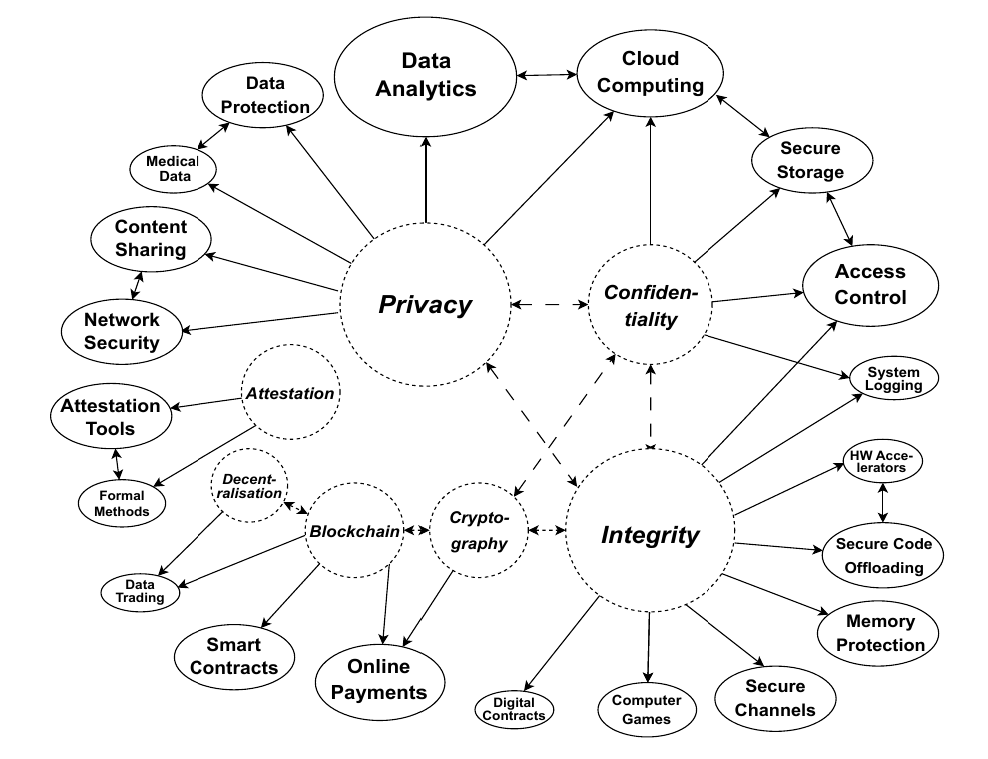
\includegraphics[scale=.3]{tee_apps.png}
    \caption{An overview of the most common TEE application use cases and
        related security properties \cite{tee_app_rev}}
    \label{fig:tee_apps}
\end{figure}

\subsection{Application Development}

There are a number of available SDKs that aid in the
development process of trusted applications. The majority of the surveyed SDKs,
support either Intel SGX, or ARM TrustZone, namely ``21 of the 23 referred
frameworks''\cite{tee_app_rev}. There are also two development tools which
offer support for RISC-V, namely Keystone \cite{tee_keystone} and Sanctum
\cite{tee_sanctum}, the latter of which appear to not be in development any
longer. With regards to programming language support, the vast majority support
either C or C++, but there are some exceptions. OP-TEE \cite{optee} also offers
support for Rust, among others like Edgeless RT \cite{edgelessrt} which also
supports Go. The Samsung Knox SDK \cite{knox_sdk}, but also open source
projects like Trusty TEE \cite{trustytee} offer Java support for the
development of Android apps.

Developers are restricted in their choice of SDK by the platform they're
developing for. Most Android TEE-enabled devices use ARM chips, and will thus
need a solution designed for ARM TrustZone \cite{arm_tz}. This resulted in
developers being constrained to use proprietary tools such as Samsung Knox SDK
\cite{knox_sdk}. However, frameworks such as OP-TEE \cite{optee} and Trusty TEE
\cite{trustytee} might be viable open source alternatives for mobile
application development. Despite the many open-source options available, their
platform support, is yet limited.

\subsection{Trusted Containers}

Adapting an application to run inside a TEE requires a lot of development
effort for making framework-specific changes. Generally, frameworks are
architecture specific. This, in turn, means that supporting a TA on multiple
architectures is a very difficult task. Trusted Containers (tcons) aim to
bridge this gap in TA development. Tcons come in as solutions which either
enable an application to run unmodified inside a TEE, or enable automatic code
modification of the application, such that it can run in the TEE. The downside
of tcons, from a security perspective, is that they increase the TCB. From a
development standpoint however, the trade-offs could be worth it, considering
the lower amount of resources invested in porting the application to run on a
TEE and the fact that some applications have limited amount of system
interactions (eg. ML models) which, as a result, diminishes their attack
surface. A non exhaustive list of the surveyed tcons include: Twine, Gramine,
vSGX, Apache Teaclave and Occlum. 

Out of all the containers analysed, none support ARM TrustZone, which further
confines mobile developers to using SDKs. Intel SGX is the most supported
architecture with 19 out of 20 projects supporting it. Only a few of them also
support AMD SEV. There are recent solutions which offer support for both
platforms, such as vSGX \cite{vsgx}. Such solutions can further simplify
development by enabling an application to run unmodified on different TEE
architectures.

LibOS \cite{libos} is a solution which was first used ten years before the
concept of TEE. Its purpose is to be an intermediary between the OS and the
client, by exposing OS functionality through a set of libraries. LibOS is
useful in the context of TEEs and tcons especially, because Intel SGX restricts
system calls inside the enclave. Because of that, unmodified applications
cannot run inside an SGX enclave, but through LibOs, system calls from inside
the enclave can be securely relayed to the OS outside of the enclave. There are
further advantages of using LibOS such as smaller TCB as a result of OS
encapsulation and increased performance as a result of a reduction in context
switches.

Wrappers around the libc library, or the WebAssembly System Interface (WASI)
act similarly as application middleware interfaces and relay system calls
outside the enclave \cite{understanding}. EGo SDK is an example utilising a
libc-wrapper, whereas AccTEE, ApacheTeaclave, or Twine use the WASI, which
enable the execution of Web Assembly (WASM) binaries inside the TEE through a
runtime for WASM.

\section{Hardware-based TEEs}

There has been a lot of research and development effort put into TEEs in the
recent years. The most common types of TEEs are based on architecture-specific
hardware extensions which enable the creation of enclaves. These will be the
focus of this section. There are both commercial and academic solutions
implemented, spanning across all major computer architectures (Intel, AMD, ARM,
POWER, RISC-V) and even more niche ones (SPARC, OPEN-RISC). It has been shown
in a previous survey that despite different approaches in design, there are
four security principles common among all implementations: \emph{verifiable
launch}, \emph{run-time isolation}, \emph{secure storage}, \emph{trusted IO}
and \emph{secure storage} \cite{tee_hw_sup}. An overview of these building
blocks can be seen in Figure \ref{fig:tee_components}.

\begin{figure}[h]
    \centering
    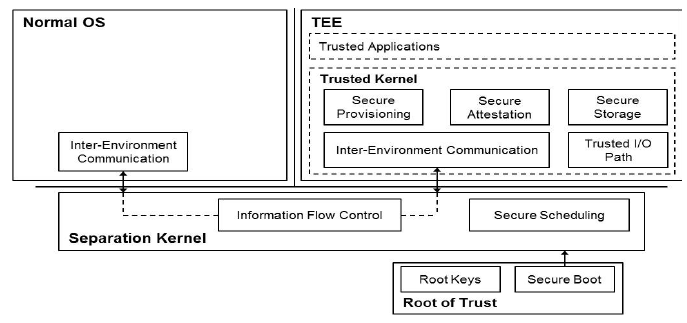
\includegraphics[scale=.6]{tee_components.png}
    \caption{An overview of TEE building blocks \cite{tee_is_and_not}}
    \label{fig:tee_components}
\end{figure}

\subsection{Verifiable Launch}

Before the enclave is even launched into execution, an important first step
must be accomplished. \emph{Verifiable launch} aims to ensure that the initial
state of the environment matches the expected state. It must also confirm that
the initial configuration is correct. 

\subsubsection{Root of Trust (Measurement).}
\label{rot}

The base of this process is an entity called \emph{Root of Trust (RTM)}. It is
the anchor of trust for the process of measurement, thus it is assumed to be
secure by design. In this context, trust is defined as the property of a system
to match its expected state of being secure. There are three types of RTMs used
by TEEs:

\begin{itemize}
    \item Static RTM (SRTM) (TMP \cite{tee_tcg_arch_overview},
        Secure Boot \cite{windows-driver-content2023Dec}) is obtained
        through an uninterrupted \emph{chain of trust} from boot time
        (reset) until the first line of code that runs in the enclave. The
        chain will generally include all software in the TCB, but not the
        OS (as it is considered untrusted software by default). It can be
        implemented in hardware directly, or as immutable software. The
        downside of SRTM is that it cannot guarantee anything about the
        state of the system mid-runtime, because it can be subject to
        cyberthreats after boot \cite{tee_smart_rot} \cite{tee_hw_sup}.
    \item Dynamic RTM (DRTM) run without trusting any prior execution. They are
        based on various architectural extensions that are meant to protect
        against adversaries that may exist on the system upon the start of the
        enclave. After all active processes are suspended and IO devices are
        disabled, a signed module is loaded, measured and authenticated. This
        will serve as the TCB and will be responsible for loading and measuring
        the enclave \cite{tee_hw_sup}.
    \item Hardware RTM (HW) can attest that a software module is not tampered
        and can be securely executed, without relying on any software. It is
        not a common implementation, but proposals such as Sancus
        \cite{tee_sancus}, or Iso-X \cite{tee_isox} exist. 
\end{itemize}

Out of the 31 implementations analysed in the survey, only a few
of them implement DRTM, some of them being commercial solutions from Intel and
AMD (\cite{arm_tz}, \cite{intel_tdx}, \cite{intel_sgx}). The rest, and the
vast majority of the academic solutions use variants of SRTM. Only one proposal
uses HW.

\subsubsection{Measurement.}

Regardless of design, each RTM involves a trusted chain of execution, where
each component \emph{measures} the next one in the chain, before passing on
execution. The measurement process consists of building a chain of
cryptographic hashes that are then securely stored. Components in the chain are
in practice also integrity checked \cite{tee_hw_sup}. This process is typically
done in a mutable part of the software TCB with a few exceptions
\label{hw_exp} such as Sancus \cite{tee_sancus} and Iso-X
\cite{tee_isox}.

\subsubsection{Attestation.}

\emph{Attestation} is the process of ensuring that upon the launch
of the newly created enclave, its state, measurement, and its
whole TCB correspond to their reference values. This is done by a
\emph{verifier}, which splits the process into: \emph{local
attestation} and \emph{remote attestation}, base on the location
of the verifier. They usually differ by the method of encryption
used, the remote verifier commonly using \emph{public key
cryptography}, while a verifier co-located with the enclave will
use \emph{symmetric key cryptography}, which is lighter on
resources. Most of the analysed solutions use remote attestation,
and only a few of them also support local attestation, concluding
thus that remote attestation is the standard both in industry and
in academia \cite{tee_hw_sup}. Like measurement, attestation is
also done in software with the same few exceptions seen in
\ref{hw_exp}.

\subsubsection{Provisioning.}

\emph{Provisioning} secrets into the newly created enclave is an optional step
that can be accomplished and is usually done as a last step, or before the
attestation. In case the provisioning is performed before the attestation, the measurement will also reflect the inclusion of the secrets. \cite{tee_hw_sup}

\subsection{Run-Time Isolation}

The resources in use by the enclave after it starts must be protected against
tampering, or reading by adversaries. These resources include the \emph{CPU}
and \emph{memory / caches}. As noted in \cite{tee_hw_sup}, we can categorize
run-time isolation by the method of \emph{partitioning} resources into a scale
from \emph{spatial} partitioning to \emph{temporal} partitioning. Extremes are
unusual, so a middle ground called \emph{spatio-temporal} partitioning is a
common choice. Isolation enforcement is categorised into \emph{logical
isolation} and \emph{cryptographic} isolation.

\subsubsection{CPU isolation.}

When analysing these strategies for CPUs it has been noted that the majority
are suboptimal. Spatial separation would involved dedicating CPU cores to
specific enclaves, which would inherently limit the total number of possible
simultaneous enclaves. A mixed, spatio-temporal solution is also sub-optimal
because of implementation difficulties. This solution would require extra
hardware in order to guarantee the integrity of spatially-separated resources.
On the other side, cryptographic enforcement would incur large computational
overhead and would likely require extra hardware. With these considerations,
the optimal solutions for CPU isolation would be the logical enforcement of a
temporal partitioning \cite{tee_hw_sup}.

The analysis shows this is indeed the case with all analysed TEEs. This is
achieved through secure context switching during which the state of the enclave
is saved, the registers of the CPU are cleared and the state of the next
enclave is loaded. The \emph{TCB} is responsible for this process and must
ensure that there is no data leakage during the context switch. To achieve a
secure context switch the \emph{TEE} relies on a combination of \emph{privilege
levels} and \emph{architectural extensions}. Most commercial solutions have
introduced new processor execution modes in support of TEEs: Intel SGX -
\emph{Enclave mode} \cite{intel_sgx}, Intel TDX - \emph{SEAM mode}
\cite{intel_tdx}, ARM CCA - \emph{Secure Mode} \cite{arm_cca}, IBM PEF -
\emph{Secure Mode} \cite{ibm_pef}. Academic solutions take a different
approach, and rely on firmware running at a higher privilege level. To ensure
that the TCB can implement the necessary security mechanisms needed
(attestation, measurement, isolation, etc.) it usually runs at higher privilege
levels, compared to the \emph{trusted applications (TA)} or VMs that run in the
enclave, which typically are executed at lower privilege levels
\cite{tee_hw_sup}. 

\subsubsection{Memory Isolation.}
\label{mem_isolation}

This is a very challenging task as part of a TEE architecture, as it involved
protecting not only the memory itself, but also various micro-architectural
structures holding recent code, branch predictions, or recent instructions.
Another important consideration the implementation of virtual address
translation into physical addresses.

By employing the same categorisation criteria, it's been observed that
successful TEE implementations use a diverse range of partitioning strategies.
Spatial partitioning implies assigning at system boot an area of memory to be
used only by the enclave or the TCB, which works well for a low number of
enclaves which have static and predictable memory requirements. Spatial
partitioning is also often leveraged to protect access control information.
Temporal isolation is the most rarely used strategy, because the context
switching is very computationally expensive, making it not suitable for systems
running concurrent enclaves. The preferred solution is the mixed
spatio-temporal partitioning as it enables dynamic reallocation of partitions
based on runtime requirements. Logical enforcement of isolation is based on an
\emph{access control mechanism} \label{acc_control} to only give access to
trusted entities. Integrity can be achieved efficiently and requires minimal
information for each enclave. Cryptographic enforcement is very strong in the
sense that it ensure confidentiality, integrity and can protect against
\emph{replay attacks} \cite{tee_replay_attacks}. However, they come at the cost
of higher storage and computation overhead, making it hard to scale. Distinctly
from the other isolation strategies, cryptographic isolation can counter an
adversary which leverages specialised hardware to perform a \emph{man in the
middle} attack at the BUS level \cite{tee_hw_sup} \label{bus_crypto}.

In practice, there are clearly preferred paths of implementation. Most
solutions Use logically enforced spatio-temporal isolation for enclave memory
and logically enforced exclusively spatial isolation for the TCB. As stated
earlier, there are also implementations that use different strategies.
\emph{Flicker} \cite{flicker} and \emph{SEA} \cite{sea_minimal_tcb} use
logically enforced temporal isolation for the both the enclave memory and the
TCB. Among others, SEV \cite{amd_sev} by AMD and AEGIS \cite{aegis}, use
cryptographically enforced spatio-temporal isolation for the enclave's memory.
The latter uses the same strategy for isolating the TCB. All sampled
implementations, however enforce the isolation via cryptographic means at the
BUS level \ref{bus_crypto}.

\subsubsection{Architectural details of memory isolation.}

Logical enforcement of spatio-temporal isolation is achieved through
\emph{access control mechanisms} as seen in \ref{acc_control}. The surveyed
TEEs use either \emph{memory protection units (MPU)} or \emph{memory management
units (MMU)}. MPUs check access rights against physical addresses of memory and
can typically offer coarse-grained memory control. This is achieved by
enforcing a limited set of access control rules, which must be managed by the
TCB. MPUs are preferred in academic solutions and are seen in modern TEEs such
as Sancus \cite{tee_sancus}, Keystone \cite{tee_keystone}, or CURE
\cite{tee_cure}. MMUs offer more fine grained control. MMUs handle virtual
addresses and convert them to physical addresses via page tables. Entries in a
page table also hold sensitive information which must be protected (eg. access
permissions). This is achieved either by letting the TCB managed all page
tables of the enclaves as well as the page tables of all \emph{untrusted
software} \cite{tee_ha-vmsi}, or by having the TCB manage only the tables of
the enclaves and then using additional access information for enclave access,
based on the execution context \cite{intel_tdx}, \cite{arm_tz},
\cite{arm_realms} \cite{tee_hw_sup}.

\subsubsection{Caches.}

Caches store recently accessed data to improve performance and have been
notoriously been used for leaking data, as will be further seen in
\ref{cache_attacks}. Enclave data can be protected in the cache by using
functions of the MMU / MPU, as seen in some architectures \cite{intel_sgx}. In
others, this is achieved with additional protection strategies \cite{arm_tz}.
Most of the solutions involved logically enforced spatio-temporal isolation of
the caches, but there are exceptions, mainly aiming to mitigate side-channel
attacks \ref{sidechannel_attacks}. Spatial partitioning, despite not scaling
well and diminishing performance is implemented for example in MI6
\cite{tee_mi6}, or Keystone \cite{tee_keystone}. Temporal partitioning involves
flushing the full cache on each context switch, which drastically degrades
performance, but from the same prior considerations it is used in a few
implementations such as SANCTUARY \cite{tee_sanctuary}, or Sancus
\cite{tee_sancus}. No cryptographic solution for isolation has been used for
caches, most likely because of the increased latency it would result in
\cite{tee_hw_sup}.

\subsection{Secure Storage}

\emph{Sealing} is defined as the process of protecting state data across different 
instances of the same enclave, through encryption. \emph{Unsealing} is the opposite 
of sealing.

As a result of the survey, it's been determined that all TEE solutions that
explicitly describe their design choices for secure storage follow closely the
sealing algorithm from of a Trusted Platform Module (TPM)
\cite{trust_plat_mod}, an immutable hardware component. An asymmetric key pair
used to encrypt a secret. The secret will only be unsealed if the system state
matched the state at the time of sealing. Further, the secret is used for
decrypting the stored data. Solutions such as SEA \cite{sea_minimal_tcb}, or
IBM-PEF \cite{ibm_pef} are based on a TPM microcontroller. Intel SGX
\cite{intel_sgx} exposes sealing capabilities through CPU instructions. There
are however, solutions which provide sealing support purely thought their
software TCB, such as \cite{optee}, or \cite{tee_timber}. This is useful in
solutions which utilise a software TCB, as it it not dependant on the system's
hardware \cite{tee_hw_sup}.

\subsection{Trusted IO}

In the context of of TEEs, \emph{Trusted IO} refers to the secure interaction
between enclaves and external devices and has two components: \emph{trusted path},
and \emph{trusted device architecture}.

\subsubsection{Trusted Path.}

A \emph{trusted path} is a secure communication channel that ensures
confidentiality and integrity of enclave's access to the device. It can be
established either through logical or cryptographic means.

Logical trusted paths require architectural support for direct memory access
(DMA) and memory mapped IO (MMIO). The former involves the same techniques used
to protect memory access in an enclave (see \ref{mem_isolation}). A trusted path for
MMIO can be implemented by allowing or denying MMIO requests based on source or
destination. This can be achieved through access filters. A number of
implementations leverage the \emph{Trusted Protection Controller} from ARM for
this task \cite{tee_truz_droid}, \cite{tee_vbutton}. Solutions such as CURE
\cite{tee_cure} and HECTOR-V \cite{tee_hector_v} use more complex filters in
from of each IO device. As seen in \ref{mem_isolation}, MPUs can be used to
create secure memory mappings, which can be used to build trusted paths between
enclaves and IO devices.

Cryptographic trusted paths are based on encryption and create a secure
communication channel between the enclave and the device, which must be both
provisioned with credentials and cryptographic keys for authentication. As
previously mentioned, these solutions come with a computational overhead, but can also
bring the advantage of protection at the link level. There are a number of TEEs
which utilise cryptographic trusted paths either solely (eg. HIX
\cite{tee_hix}), or in combination with logical trusted paths (eg. SGXIO
\cite{tee_sgxio}).   

\subsubsection{Trusted Device Architecture.}

There are some devices that do not process confidential data in clear text for
which only a \emph{trusted path} is suffices. However, there are are devices
that gained traction in the last year which make computations on user data, and
which must ensure confidentiality and integrity of the enclave's data. Examples
of such devices are GPUs, dedicated AI chips, or FPGAs. Since the devices
differ significantly in architecture, only a high-level overview of the
implementation strategy could be covered \cite{tee_hw_sup}. Temporal
partitioning of the IO device is a common strategy and requires a secure
context switch. Examples include HEETEE \cite{tee_heetee} for generic
accelerators, HIX \cite{tee_hix} for GPUs and ShEF \cite{tee_shef} for FPGAs.
Logically enforced temporal partitioning is also a common solution when
multiple enclaves need to access a resource concurrently. This is typically
achieved through an architecture specific mechanism of partitioning resources
to enclaves and keeping track of ownership. Recent proposals include SEGIVE
\cite{tee_segive} for GPUs and TrustOre \cite{tee_trustore} for FPGAs. Spatial
partitioning and cryptographic enforcement are considered unsuitable
\cite{tee_hw_sup}.

\section{Other Architectures}

The vast majority of relevant academic and industry TEE implementations used
hardware extensions to provide the necessary building blocks for TEEs. There
exist however some architectures that diverge from this trend.

Purely software-based architecture try to address the dependence of TEEs on the
CPU architecture of the system they are running on. A relevant example is
SecTEE, which implements in its software TCB all primitives necessary for
running secure enclaves: ``integrity measurement, remote attestation, data
sealing, secrets provisioning, and life cycle management'' \cite{sec_tee}.

On the other hand, we find solutions such as AMD Platform Security Processor
(PSP), Google Titan M, Apple Secure Enclave Processor (SEP) or Hardware
Security Modules (HSM), which aim to provide similar benefits with TEEs, but
are implemented as separate chips from the main CPU.

\section{Vulnerabilities}

This section is based on a recent survey by Muñoz et al.
\cite{tee_in_securities}, and will provide an overview of vulnerabilities in
TEEs as well as a number of examples for each category.

\subsection{Software vulnerabilities}

In spite of the security mechanisms introduced by TEEs, the software running on
the system is still often vulnerable. Unintentional bugs that have previously
been found in the code of TAs running inside enclaves can include improper
parameter validation, or improper memory handling. Attacker can exploit such
vulnerabilities and compromise the system with effects ranging from revealing
sensitive information to exploiting the kernel of the TEE.

\subsubsection{Kernel attacks.}

There are a number of Kernel exploits performed on TEEs. Most of them involve a
multi-step process, chaining together exploits on different components. As
described by the authors, these exploits can include applications running the
NW that communicate with the TEE, attacks on vulnerable TEE drivers, privilege
escalations, disabling of protection mechanisms, vulnerable syscalls, etc. It
has been proven in the past that an attacker can get full control over any
aspect of a device through such methods, in exploits such as \emph{Bits Please}
\cite{bits_please}. 

\subsubsection{System calls.}

A number of attacks exploit vulnerabilities in the implementation of system
calls in the TEE. Techniques such as the aforementioned ones can be utilised
to gain higher privileges through a vulnerable trusted application. Then the
vulnerable system call can be exploited, for example to extract encryption keys
from the system \cite{bits_fde}. Another example involves the lack of user
input validation in certain system calls. \emph{Trust None} \cite{trust_none}
exploits this to bypass certain security mechanisms which leads to read and write
permissions in the TZ kernel context. Bootloader unlocking has been proven 
possible through this exploits.

%\subsubsection{Downgrade Attack.}

% TODO include architectural attacks or not?
% -- erring on the side of NOT

%Trusted applications must be signed using the TEE trusted public key, meaning that 
%an application will pass verification if it's properly signed. The Downgrade attack
%involved executing older versions of a TA, known to be vulnerable. These can then be
%exploited in order to hijack control of the system. To mitigate this, a versioning
%system was introduced. However, research shows that adoption of the system was slow,
%so despite mitigations being introduced, they can be rendered useless by lack of adoption.

\subsection{Side-channel attacks}
\label{sidechannel_attacks}

\emph{Side Channel attacks} (SCA) mainly exploit secondary sources of
information (power consumption, noise levels, response time, etc.) to extract
information from a system. A subcategory of SCAs, called \emph{Fault Injection}
(FI) exploit glitches induced by applying high voltages, temperatures, or
electromagnetic pulses. FI attacks are particularly hard to protect against.

\subsubsection{PlunderVolt.}

Plundervolt \cite{plundervolt} involves a privileged adversary which abuses a
voltage scaling interface to cause predictable failures in the system. PlunderVolt
can break the confidentiality and integrity of data in Intel SGX, despite memory
encryption. Event more, PlunderVolt can be exploited to alter the Instruction Set
of the processor, thus making it possible to attack previously trusted, bug free
code.

\subsubsection{Platypus.}

Intel exposes to unprivileged users and interface which reveals power
consumption. Platypus \cite{platypus} shows that this information can be
leveraged through various statistical techniques to identify code instructions
and thus monitor application control flow. Moreover, researchers showed that
Platypus can be leveraged to infer secret keys, break KASLR \cite{kaslr} and
create a covert channel through which information can be leaked from inside
enclaves.

\subsection{Micro-architectural attacks}

Attacks falling in this category target micro-architectural elements and
execution processes, which include among others: cache memory, the branch
predictor and out-of-order execution.

\subsubsection{Cache timing attacks.}
\label{cache_attacks}

TEEs based on TrustZone (TZ) have been shown vulnerable to cache timing
attacks. On such systems, the cache is shared between the NW and the Secure
World. As a result, attackers can exploit hardware information such as access
time on cache lines to extract information from enclaves. The most common
target is encryption keys. Successful deployments of these attacks showed
several weaknesses in the NS-bit mechanism in TZ, which separates the SW from
NW. Such attacks, have also been shown possible on Intel SGX. In fact, the
authors affirm that SGX increases the side-channel attack surface
\cite{cache_sgx} of Intel systems. Concrete examples of cache timing attacks
include Prime+Probe \cite{prime_probe}, Flush+Reload \cite{flush_reload} and
Flush+Flush \cite{flush_flush}.

\subsubsection{Speculative execution attacks.}

Speculative execution is an optimization mechanism present in all modern CPUs.
It is based on predicting future execution flow (speculation) and executing the
predicted set of instructions in advance. In case the prediction was wrong, the
state is reverted. However, not all changes are reverted and speculative
execution can leave traces behind, which can be leveraged by attackers to
extract confidential information, despite security measures protecting it.
Meltdown and Spectre are the two most prevalent example of speculative
execution attacks and have been shown possible on Intel SGX and ARM TZ
\cite{brasser}, \cite{sgxpectre}.

\subsubsection{Out-of-order execution attacks.}

As a subtype of speculative execution, out-of-order executing allows
instructions to be executed out of order to maximize performance. There are a
number of attacks which exploit this behaviour. Foreshadow \cite{foreshadow}
proved that Intel SGX is not resistant against speculative execution attacks,
by reading memory inside the enclave and extracting attestation keys.
Micro-architectural data sampling (MDS) attacks also fall in this category.
These, typically involve the exfiltration of data from internal CPU buffers.
A notable instance for this type of attack is Fallout \cite{fallout}.

%TODO include mitigations?

\section{Conclusions}

Trusted execution environments have been increasingly adopted in the past few
years as a mechanism for providing security features in the context of
computing devices, from mobile to cloud. In this paper we gave an overview of
TEE, covering three main topics.

Firstly, we discussed their most common use cases seen until now, which include Data
Processing, Finance and Authentication. We also analysed the tools currently
used in order to develop Trusted Applications. The options are mostly limited
to Intel SGX and ARM TrustZone. Furthermore, the cross-platform options are
very limited. Tcons, which try to avoid platform-specific modifications in the
development process, have also been briefly covered.

Secondly, we discussed in detail the four security principles which are common
among all implementations of hardware-based TEEs, namely: \emph{verifiable
launch}, \emph{run-time isolation}, \emph{secure storage}, \emph{trusted IO}
and \emph{secure storage}. We also briefly covered other types of
architectures.

Thirdly, we covered a number of relevant types of exploits encountered in the
realm of TEEs including software-based, side-channel-based and
micro-architectural attacks. The goal of TEEs is to provide higher security
guarantees for TAs as opposed to ``classic'' applications. However, the vast
number of ways TEEs have been attacked proves that they are not a bullet-proof 
solution and still have a number of security shortcomings.

TEEs are a good solution in the development of more secure applications, but
they still are an immature technology which will likely continue to improve
in the near future, addressing development and security issues.

\newpage

\bibliographystyle{splncs03}
\bibliography{sesebib.bib}

% Declaration {{{

%% -------------------
%% |   Declaration   |
%% -------------------
\cleardoublepage
%\vspace*{5\baselineskip}
\hbox to \textwidth{\hrulefill}
\par
%\iflanguage{english}{english text here}{german text here}

\noindent Ich versichere, dass ich die vorstehende Arbeit selbstständig und ohne fremde Hilfe angefertigt und mich keiner anderer als der in den beigefügten Verzeichnissen angegebenen Hilfsmittel bedient habe.
\textbf{Außerdem erkläre ich ausdrücklich, dass für die vorliegende Arbeit, mit Ausnahme reiner Übersetzungs- und Grammatiktools, keine text- und mediengenerierenden KIs (wie ChatGPT) oder ähnliche elektronische Programme zum Einsatz kamen.}
Alle Textstellen, die wörtlich oder sinngemäß aus Veröffentlichungen Dritter entnommen wurden, sind als solche kenntlich gemacht.
Alle Quellen, die dem World Wide Web entnommen oder in einer digitalen Form verwendet wurden, sind der Arbeit beigefügt.
\bigbreak
\noindent Weitere Personen waren an der geistigen Leistung der vorliegenden Arbeit nicht beteiligt.
Insbesondere habe ich nicht die Hilfe eines Ghostwriters oder einer Ghostwriting-Agentur in Anspruch genommen.
Dritte haben von mir weder unmittelbar noch mittelbar Geld oder geldwerte Leistungen für Arbeiten erhalten, die im Zusammenhang mit dem Inhalt der vorgelegten Arbeit stehen.
\bigbreak
\noindent Der Durchführung einer elektronischen Plagiatsprüfung stimme ich hiermit zu.
Die eingereichte elektronische Fassung der Arbeit ist vollständig.
Mir ist bewusst, dass nach\-träg\-li\-che Ergänzungen ausgeschlossen sind.
\bigbreak
\noindent Die Arbeit wurde bisher keiner anderen Prüfungsbehörde vorgelegt und auch nicht veröffentlicht.
Ich bin mir bewusst, dass eine unwahre Erklärung zur Versicherung der selbstständigen Leistungserbringung rechtliche Folgen haben kann.

\vspace*{2\baselineskip}

\noindent\textbf{\place, \submissionTime}
\vspace{1.5cm}

\noindent\dotfill\hspace*{8.0cm}\\
\noindent\hspace*{2cm}(\authorName) %center name with hspace

% }}}

\thispagestyle{empty}

\end{document}
